\videotitle{Practical Recommendations for NAS and HPO}

%----------------------------------------------------------------------
\myframe{Maturity of the Fields of NAS and HPO}{
	\myit{
		\item \alert{Hyperparameter optimization is a mature field}
		\myit{
			\item[-] Blackbox HPO has been researched for decades; \\ there are many software packages
			\item[-] Multi-fidelity HPO has also become quite mature
%			\item[-] Gradient-based HPO is still a nascent field
		}
\medskip
\pause
		\item \alert{Neural architecture search is still a very young field}
\pause
		\myit{
			\item[-] Blackbox is quite mature, but slow
			\item[-] Multi-fidelity NAS is also quite mature and faster
\pause
			\item[-] Meta-learning + multi-fidelity NAS is fast, but is still a very young field
\pause
\smallskip
			\item[-] Gradient-based NAS is fast, but can have failure modes with terrible performance
			\item[-] Gradient-based NAS hasn't reached the hands-off AutoML stage yet
		}
\medskip
\pause
		\item NAS is mainly used to \alert{create new architectures that many others can reuse}
		
\medskip
\pause
		\item Given a new dataset, \alert{HPO is crucial for good performance; NAS may not be necessary}
		\myit{
			\item[-] The biggest gains typically come from tuning key hyperparameters (learning rate, etc)
			\item[-] Reusing a previous achitecture often yields competitive results
		}
	}
}
%----------------------------------------------------------------------

%----------------------------------------------------------------------
\myframe{Practical Recommendations for NAS and HPO}{
	\myit{
		\item Recommendations for a new dataset
		\myit{
			\item[$\rightarrow$] Always run HPO
			\item[$\rightarrow$] Try NAS if you can 
		}
\bigskip
\pause
		\item How to combine NAS \& HPO
		\myit{
			\item[-] If the compute budget suffices, \alert{optimize them jointly}, e.g., using BOHB
			\myit{
				\item[+] Auto-PyTorch Tabular \lit{\href{https://github.com/automl/Auto-PyTorch}{Zimmer,\,Lindauer\,\& Hutter, 2020}}
				\item[+] Auto-RL \lit{\href{https://arxiv.org/abs/1812.11951}{Runge et al, 2019}}
			}
\medskip
\pause
			\item[-] Else
			\myit{
				\item[+] If you have decent hyperparameters:\\
			\alert{run NAS, followed by HPO for fine-tuning} \lit{\href{https://arxiv.org/abs/1905.07443}{Saikat et al, 2019}}
\smallskip
\pause
				\item[+] If you don't have decent hyperparameters: \alert{first run HPO} to get competitive	
			}
%\medskip
%\pause
%			\item[-] To improve robustness of DARTS, \\
%			tune DARTS' own hyperparameters with BOHB \lit{\href{https://openreview.net/forum?id=SJx9ngStPH}{Zela et al, 2020}}
		}
	}
}
%----------------------------------------------------------------------


%----------------------------------------------------------------------
\myframe{Case Study: NAS \& HPO in Auto-PyTorch Tabular \litw{\href{https://github.com/automl/Auto-PyTorch}{Zimmer,\,Lindauer\,\& Hutter, 2020}}}{

\begin{columns}[T]
	\column{0.29\textwidth}

\onslide<1->{
	\myit{
		\item \alert{Joint Architecture Search and Hyperparameter Optimization}
		\myit{
\onslide<2->{
			\item[-] Purely using HPO techniques: very similar methods as in \alert{Auto-sklearn 2.0}
}
\onslide<3->{
			\item[-] \alert{Multi-fidelity optimization} with \alert{BOHB}
			\item[-] \alert{Meta-learning} with \alert{task-independent recommendations}
}
\onslide<4->{
			\item[-] \alert{Ensembling} of neural nets and traditional ML models
}
}
		}
	}
	
	\column{0.29\textwidth}	
\onslide<1->{
	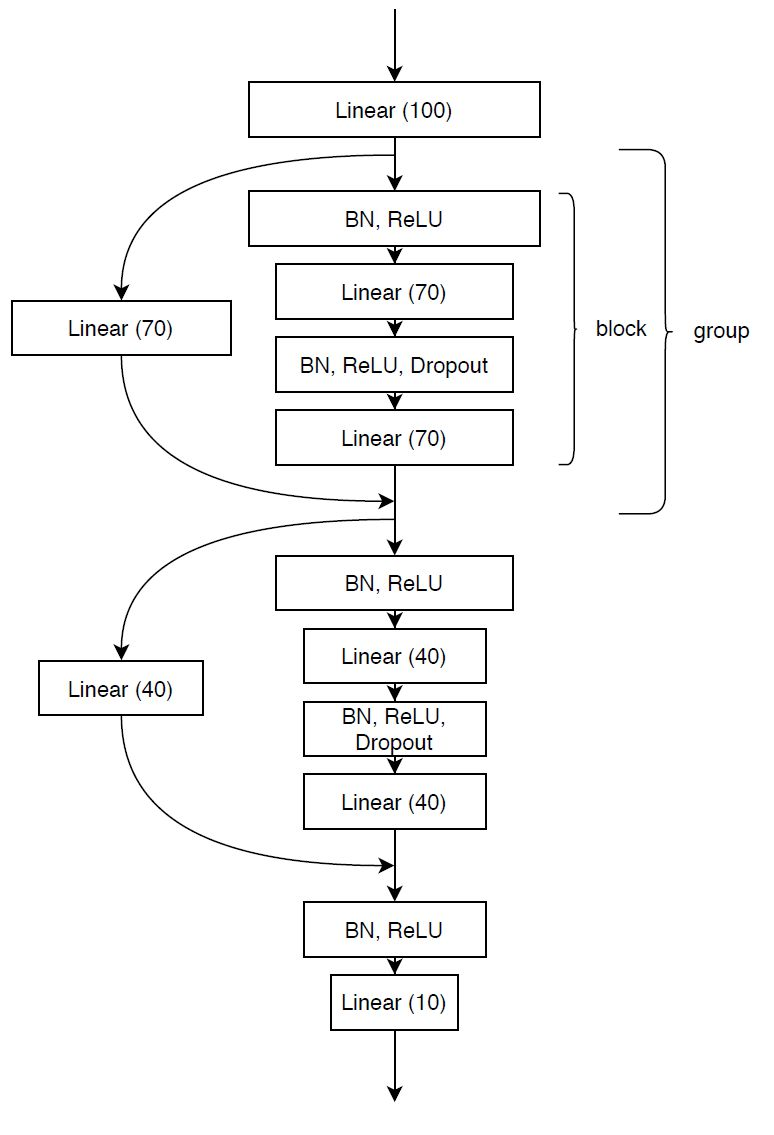
\includegraphics[width=\linewidth]{images/AutoPytorch-ShapedResNet.png}\\
}
	\column{0.42\textwidth}	
\vspace*{-0.7cm}
\onslide<1->{
	\begin{center}
	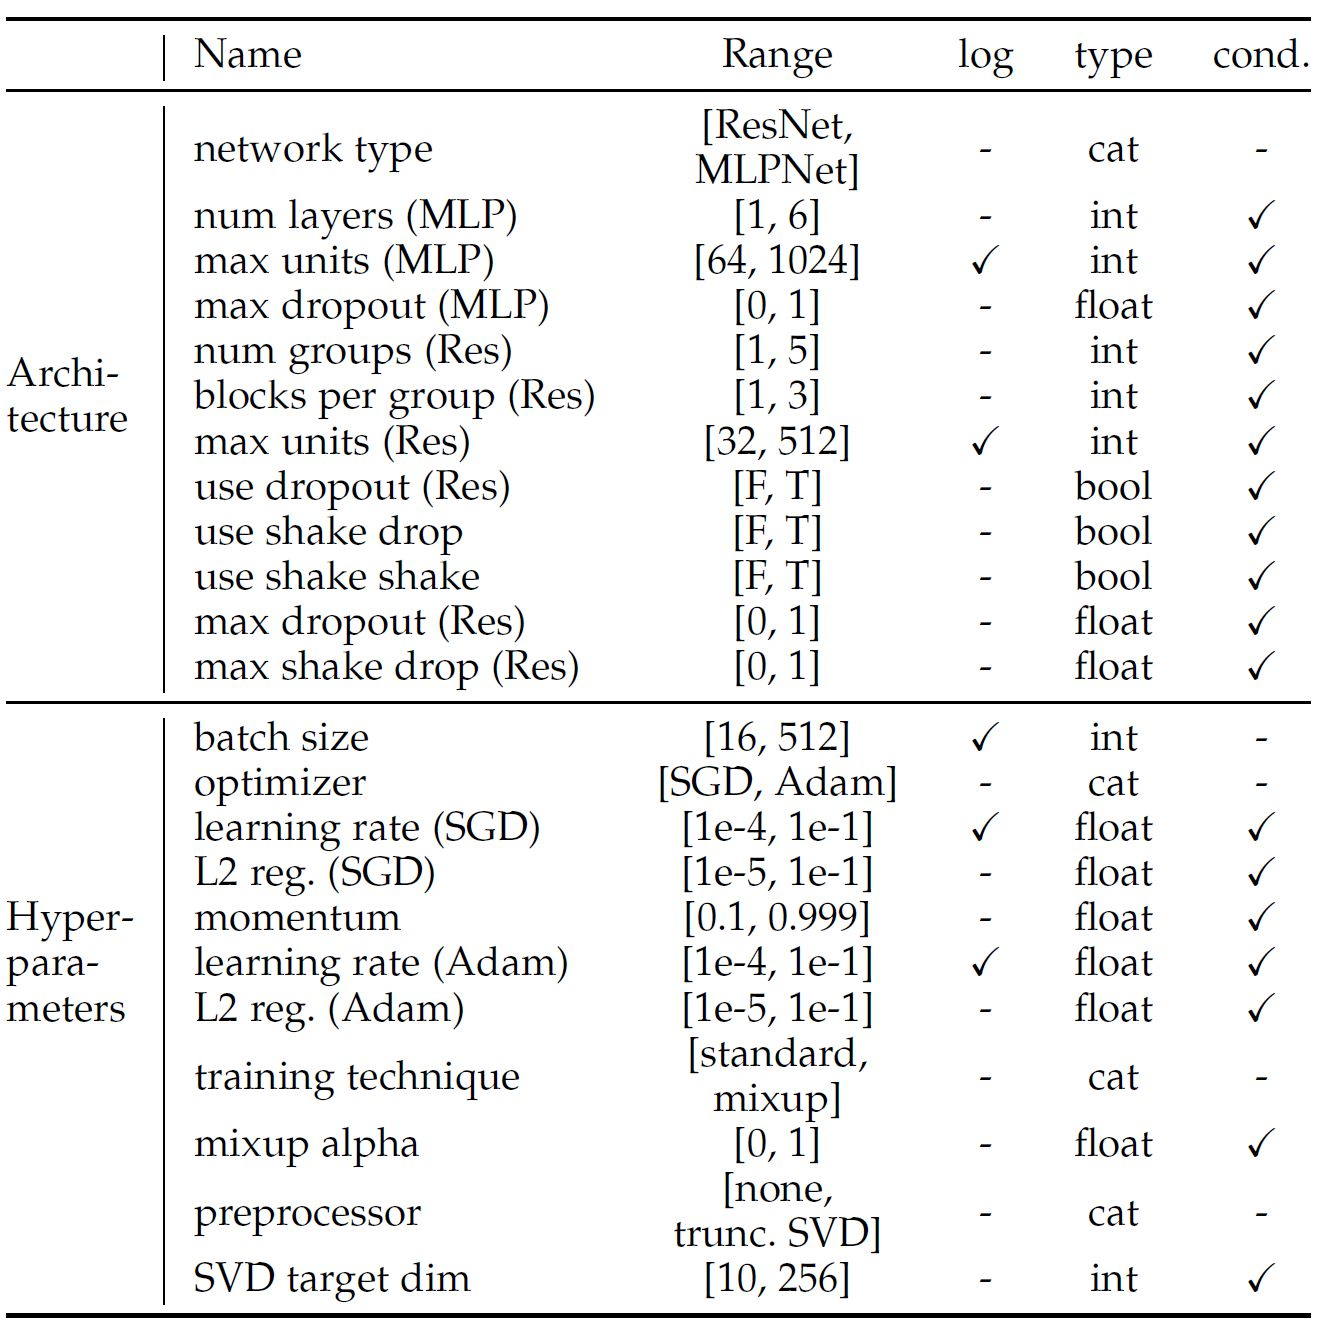
\includegraphics[width=0.9\linewidth]{images/AutoPytorch-ConfigSpace.png}
	\end{center}
}
\onslide<5->{
	\vspace*{-0.3cm}\hspace*{-1.1cm}
	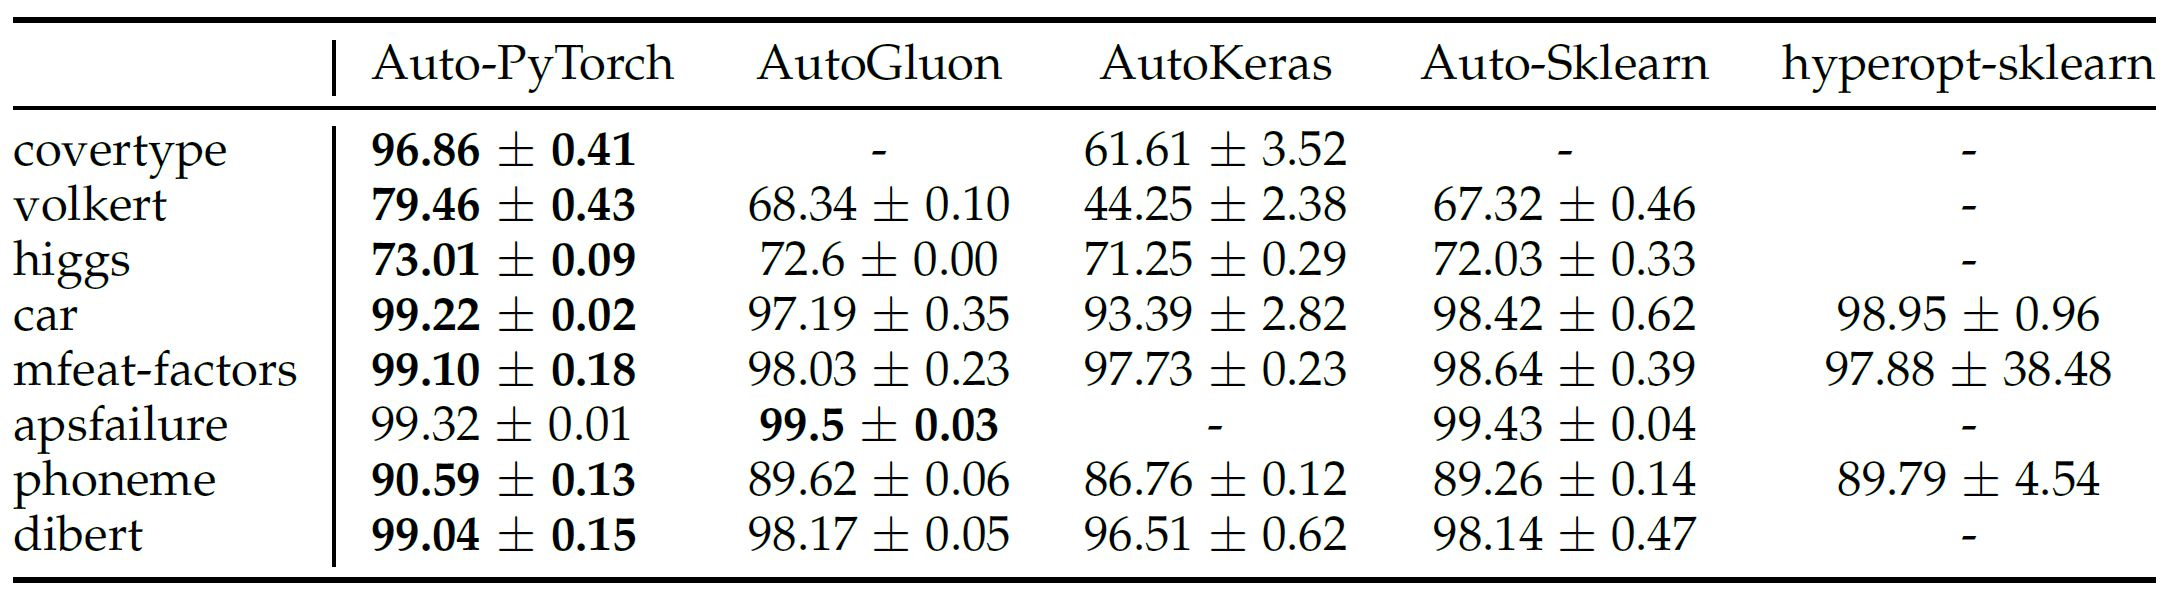
\includegraphics[width=1.1\linewidth]{images/AutoPytorch-performance.png}
%	\end{center}
}


\end{columns}
}
%----------------------------------------------------------------------


%----------------------------------------------------------------------
\myframe{Case Study: NAS \& HPO in Auto-DispNet}{
	\begin{columns}[T]
		\column{0.64\textwidth}
		\myit{
			\item Problem: disparity estimation
			\myit{
				\item[-] Estimate depth from stereo images
			}
	\onslide<2->{
	\smallskip
				\item Background: U-Net
			\myit{
				\item Skip connections from similar spatial resolution to avoid loosing information
			}
	}\onslide<3->{
	\smallskip
				\item Search space for DARTS
			\myit{
				\item 3 cells: keeping spatial resolution, downsampling, 
				and \alert{new upsampling cell that supports U-Net like skip connections} 
			}
		}
	\smallskip
	}
	\onslide<4->{
		\myit{
			\item Both NAS and HPO improved the state of the art \lit{\href{https://arxiv.org/abs/1905.07443}{Saikat et al, 2019}}:
			\myit{
				\item End-point-error (EPE) on Sintel dataset: \alert{2.36 $\rightarrow$ 2.14 (by DARTS)}
				\item Subsequent HPO: \alert{2.14 $\rightarrow$ 1.94 (by BOHB)}
			}
		}
	}

		\column{0.35\textwidth}
		\centering
		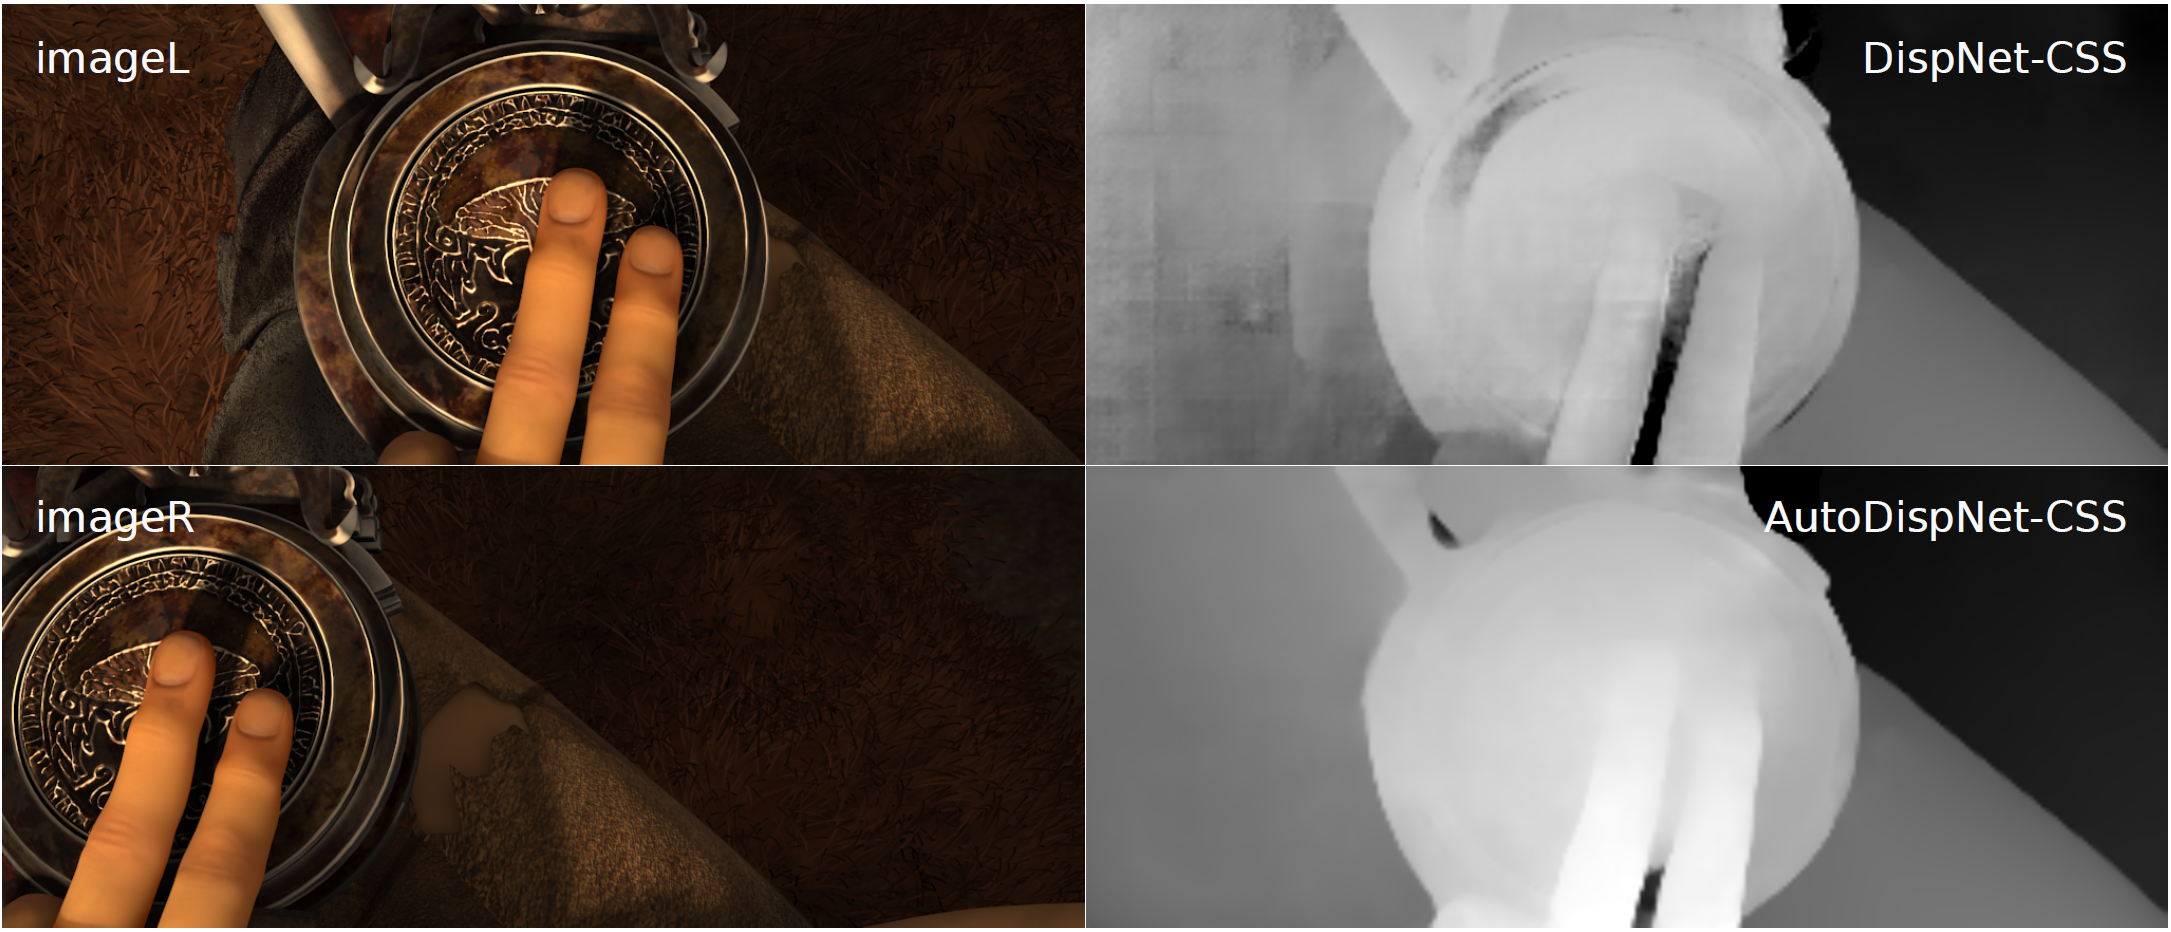
\includegraphics[width=\linewidth]{images/disparity_estimation}\\
\bigskip
\bigskip
\onslide<2->
		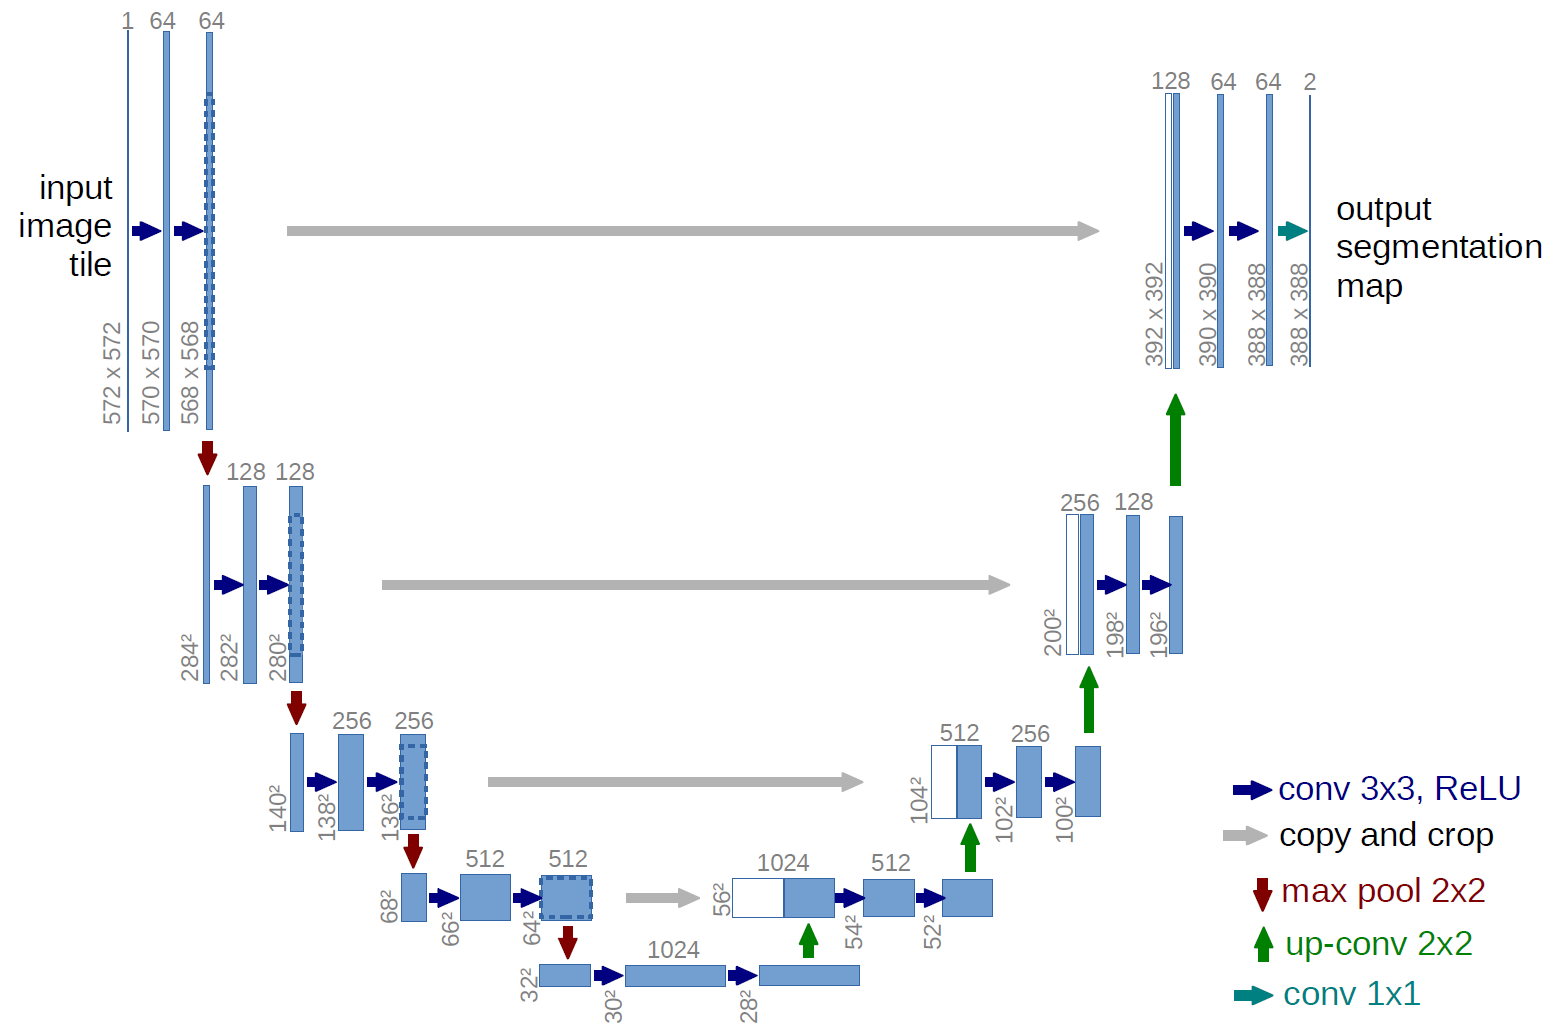
\includegraphics[width=\linewidth]{images/u-net-architecture}	 
	\end{columns}	
}
%----------------------------------------------------------------------

%----------------------------------------------------------------------
%\myframe{Case Study Details (Auto-DispNet)}{
%	\myit{
%		\item Very important: \alert{warmstarting} of the network weights
%		\myit{
%			\item First half of the training epochs: \\
%			keep one-shot architecture weights fixed to the uniform distribution
%			\item Only afterwards: \\
%			DARTS' alternating updates of weights and architectural parameters
%		}
%\bigskip
%		\item Without warmstarting:\\
%		\alert{DARTS found cells with only parameterless operations}
%	}	
%}
%----------------------------------------------------------------------



%----------------------------------------------------------------------
\myframe{Questions to Answer for Yourself / Discuss with Friends}{

	\myit{
		\item Repetition:\\ \alert{If you want to use both HPO and NAS for your problem, how could you proceed?}
\medskip
		\item Discussion:\\ \alert{Think of a problem of your particular interest. For that problem, which approach would you use to combine HPO and NAS, and why?}
	}	 
}
%-----------------------------------------------------------------------

%----------------------------------------------------------------------
%\myframe{Learning Goals}{
%
%	After this week's videos on HPO and NAS, you should be able to \ldots
%	
%	\begin{itemize}
%		\item describe \alert{several ways of speeding up over blackbox NAS}  %(except via meta-learning)
%		\item describe \alert{several ways of speeding up over blackbox NAS}  %(except via meta-learning)
%		\myit{
%			\item define \alert{network morphisms} \& \alert{explain how to use them to speed up NAS}
%			\item explain various \alert{multi-fidelity Bayesian optimization methods}
%		}
%		\item discuss \alert{when and how to use NAS and HPO in practice} 
%		\item describe \alert{failure modes of DARTS}
%	\end{itemize}
%}

